\documentclass{article}

\usepackage{amsmath}
\usepackage{tikz}
\usepackage{xepersian}

\settextfont{XB Niloofar}

\title{سیگنال‌ها و سیستم‌ها - دکتر سلیمی‌بدر}
\author{امیرحسین منصوری - ۹۹۲۴۳۰۶۹}
\date{تمرین سری ۱}

\begin{document}
	\maketitle

	\section*{سوال ۱}
	\paragraph*{}
	با ۱ واحد جابه‌جایی به چپ،
	$g(1+t)$
	به دست می‌آید:
	\begin{center}
		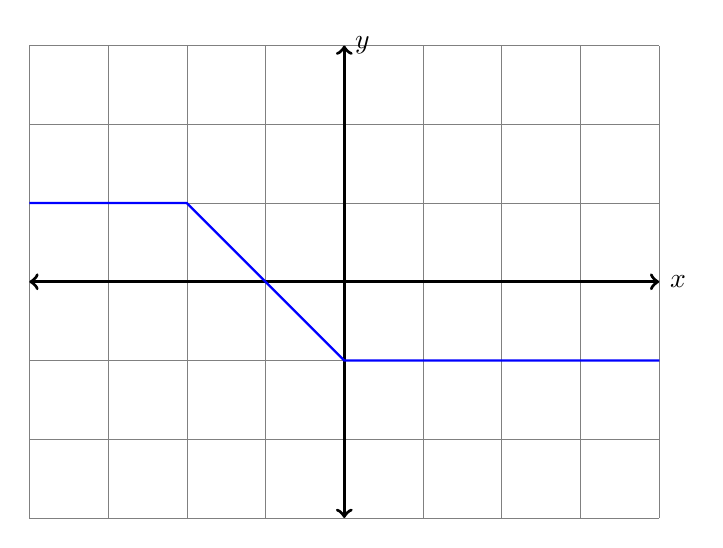
\begin{tikzpicture}[align=center]
			\draw[very thin, gray] (-4, -3) grid (4, 3);
			\draw[very thick, <->] (-4, 0) -- (4, 0) node[right]{$x$};
			\draw[very thick, <->] (0, -3) -- (0, 3) node[right]{$y$};

			\draw[blue, thick] (-4, 1) -- (-2, 1) -- (0, -1) -- (4, -1);
		\end{tikzpicture}
	\end{center}

	\paragraph*{}
	با اعمال تبدیل معکوس زمانی،
	$g(1-t)$
	به دست می‌آید:

	\begin{center}
		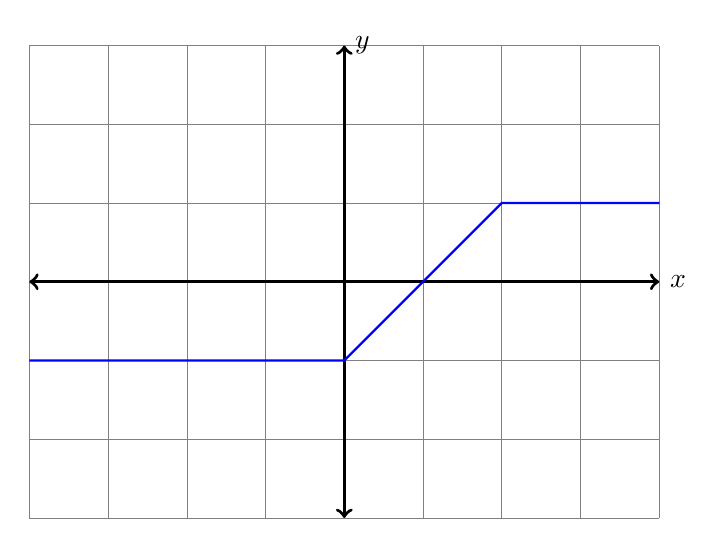
\begin{tikzpicture}[align=center]
			\draw[very thin, gray] (-4, -3) grid (4, 3);
			\draw[very thick, <->] (-4, 0) -- (4, 0) node[right]{$x$};
			\draw[very thick, <->] (0, -3) -- (0, 3) node[right]{$y$};

			\draw[blue, thick] (-4, -1) -- (0, -1) -- (2, 1) -- (4, 1);
		\end{tikzpicture}
	\end{center}


	\paragraph*{}
	با قرینه کردن نسبت به محور
	$x$ها،
	$-g(1-t)$
	به دست می‌آید:

	\begin{center}
		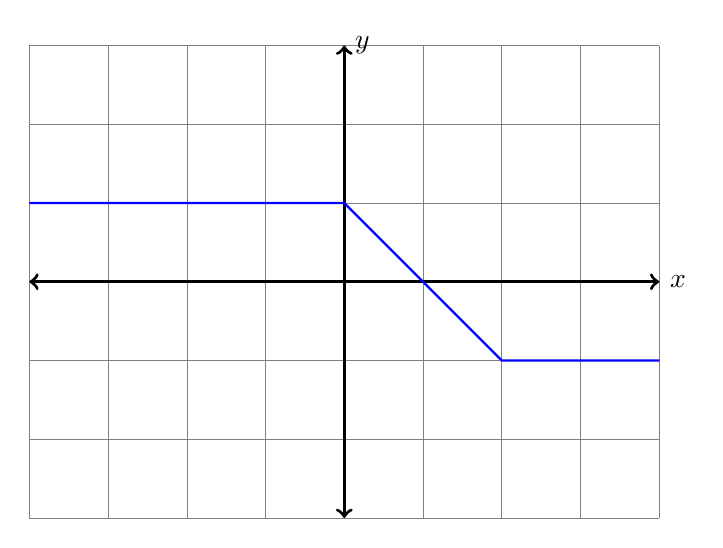
\begin{tikzpicture}[align=center]
			\draw[very thin, gray] (-4, -3) grid (4, 3);
			\draw[very thick, <->] (-4, 0) -- (4, 0) node[right]{$x$};
			\draw[very thick, <->] (0, -3) -- (0, 3) node[right]{$y$};

			\draw[blue, thick] (-4, 1) -- (0, 1) -- (2, -1) -- (4, -1);
		\end{tikzpicture}
	\end{center}

	\paragraph*{}
	با ۱ واحد جابه‌جایی به سمت بالا،
	$1-g(1-t)$
	به دست می‌آید:

	\begin{center}
		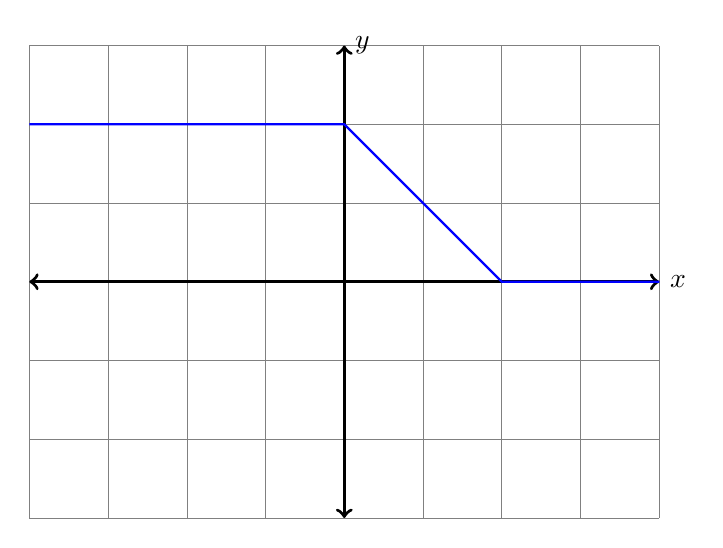
\begin{tikzpicture}[align=center]
		\draw[very thin, gray] (-4, -3) grid (4, 3);
		\draw[very thick, <->] (-4, 0) -- (4, 0) node[right]{$x$};
		\draw[very thick, <->] (0, -3) -- (0, 3) node[right]{$y$};

			\draw[blue, thick] (-4, 2) -- (0, 2) -- (2, 0) -- (4, 0);
		\end{tikzpicture}
	\end{center}

	\section*{سوال ۲}
	\paragraph*{}
	می‌دانیم
	\begin{equation*}
		x_o(t) = \frac{x(t) - x(-t)}{2}
	\end{equation*}

	\paragraph*{}
	برای به دست آوردن
	$-x(-t)$،
	نمودار
	$x(t)$
	را نسبت به مبدا مختصات، قرینه می‌کنیم:

	\begin{center}
		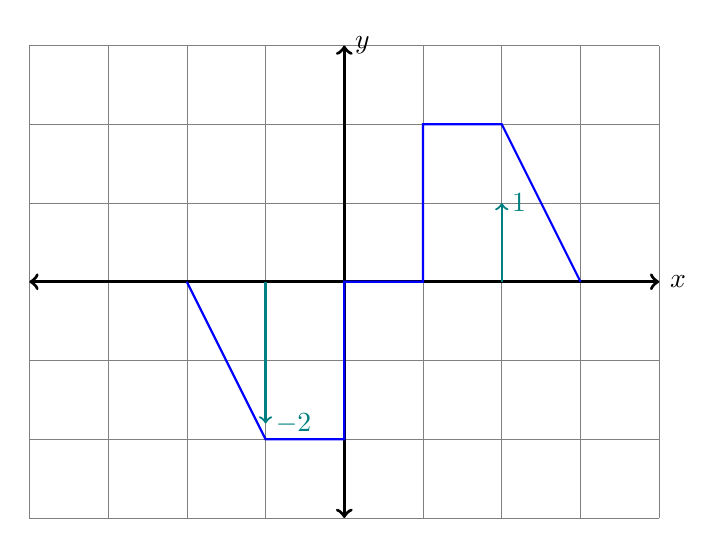
\begin{tikzpicture}[align=center]
			\draw[very thin, gray] (-4, -3) grid (4, 3);
			\draw[very thick, <->] (-4, 0) -- (4, 0) node[right]{$x$};
			\draw[very thick, <->] (0, -3) -- (0, 3) node[right]{$y$};

			\draw[thick, blue] (-2, 0) -- (-1, -2) -- (0, -2) -- (0, 0) -- (1, 0) -- (1, 2) -- (2, 2) -- (3, 0);

			\draw[thick, teal, ->] (-1, 0) -- (-1, -1.8) node[right] {$-2$};
			\draw[thick, teal, ->] (2, 0) -- (2, 1) node[right] {$1$};
		\end{tikzpicture}
	\end{center}

	\paragraph*{}
	حال می‌توانیم نمودار قسمت فرد را از روی نمودار
	$x(t)$
	و
	$-x(-t)$
	به دست بیاوریم. کافیست این دو را با هم جمع کنیم و عرض نقاط را نصف کنیم:

	\begin{center}
		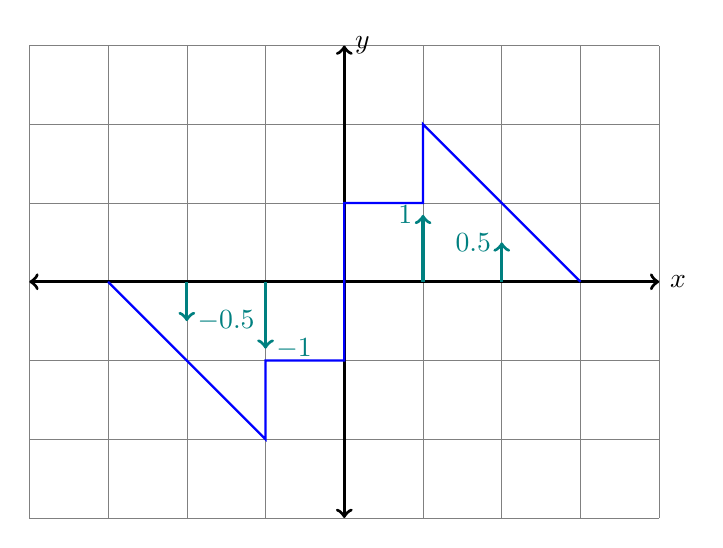
\begin{tikzpicture}[align=center]
			\draw[very thin, gray] (-4, -3) grid (4, 3);
			\draw[very thick, <->] (-4, 0) -- (4, 0) node[right]{$x$};
			\draw[very thick, <->] (0, -3) -- (0, 3) node[right]{$y$};

			\draw[thick, blue] (0, 0) -- (0, 1) -- (1, 1) -- (1, 2) -- (2, 1) -- (3, 0);

			\draw [thick, blue] (0, 0) -- (0, -1) -- (-1, -1) -- (-1, -2) -- (-2, -1) -- (-3, 0);

			\draw[very thick, teal, ->] (1, 0) -- (1, 0.85) node[left] {$1$};
			\draw[very thick, teal, ->] (2, 0) -- (2, 0.5) node[left] {$0.5$};

			\draw[very thick, teal, ->] (-1, 0) -- (-1, -0.85) node[right] {$-1$};
			\draw[very thick, teal, ->] (-2, 0) -- (-2, -0.5) node[right] {$-0.5$};
		\end{tikzpicture}
	\end{center}

	\paragraph*{}
	حال می‌توانیم انتگرال مورد نظر را حساب کنیم:

	\begin{align*}
		& \int_{0}^{\infty} x_o(t) dt \\
		&= \int_{0}^{1^-} x_o(t) dt
		+ \int_{1^-}^{1^+} x_o(t) dt
		+ \int_{1^+}^{2^-} x_o(t) dt
		+ \int_{2^-}^{2^+} x_o(t) dt
		+ \int_{2^+}^{3} x_o(t) dt
		+ \int_{3}^{\infty} x_o(t) dt \\
		&= 1 + 1 + \frac{(2 + 1) \times 1}{2} + 0.5 + \frac{1 \times 1}{2} + 0\\
		&= 4.5
	\end{align*}

	\paragraph*{}
	در بالا، حاصل هر انتگرال به سادگی از مساحت زیر نمودار مشخص شده در بالا به دست می‌آید.


	\section*{سوال ۳}

	\begin{align*}
		P(x(t)) &= \lim_{T \rightarrow \infty} \frac{1}{2T} \int_{-T}^{+T} \left|x(\tau)\right|^2 d \tau \\
		&= \lim_{T \rightarrow \infty} \frac{1}{2T} \left(
		\int_{-T}^{-10} 2^2 d \tau
		+ \int_{-10}^{+10} 4^2 d \tau
		+ \int_{+10}^{+T} 6^2 d \tau
		\right) \\
		&= \lim_{T \rightarrow \infty} \frac{1}{2T} \left(
		4(T - 10) + 320 + 36(T - 10)
		\right) \\
		&= \lim_{T \rightarrow \infty} 2 + 18 + \frac{-40 + 320 - 360}{2T} \\
		&= 20
	\end{align*}

	\section*{سوال ۴}
	\subsection*{الف)}

	\begin{equation*}
		\Omega_0 = \frac{3 \pi}{7} \Rightarrow T' = \frac{2 \pi}{\frac{3 \pi}{7}}
		= \frac{14}{3}
	\end{equation*}

	اگر سیگنال پیوسته بود، دوره تناوب آن برابر
	$T'$
	می‌شد. اما چون سیگنال گسسته است، دوره تناوب آن باید صحیح باشد. در نتیجه باید
	کوچکترین مضرب صحیح از
	$T'$
	را به عنوان دوره تناوب اصلی انتخاب کنیم. واضح است که این مضرب برابر
	$T_0 = 14$
	است.

	\subsection*{ب)}
	\paragraph*{}
	برای سیگنال
	$\cos(\frac{2 \pi}{3} t)$
	داریم:
	\begin{equation*}
		T_0 = \frac{2 \pi}{\frac{2 \pi}{3}} = 3
	\end{equation*}

	برای سیگنال
	$2\sin(\frac{16 \pi}{3} t)$
	داریم:
	\begin{equation*}
		T_0 = \frac{2 \pi}{\frac{16 \pi}{3}} = \frac{3}{8}
	\end{equation*}

	در نتیجه برای جمع این دو سیگنال، می‌توان گفت
	$T_0 = 3$.
	زیرا به نوعی ک.م.م دو عدد
	$3$
	و
	$\frac{3}{8}$
	برابر
	$3$
	است.

	همچنین برای سیگنال
	$\sin(\pi t)$
	داریم:
	\begin{equation*}
		T_0 = \frac{2 \pi}{\pi} = 2
	\end{equation*}
	در نتیجه برای سیگنال
	$z(t)$،
	تناوب اصلی برابر ک.م.م دو سیگنال قبلی است:
	\begin{equation*}
		z(t) : T_0 = lcm(2, 3) = 6
	\end{equation*}

	\subsection*{ج)}
	\paragraph*{}
	سیگنال متناوب نیست.

	\subsection*{د)}
	\paragraph*{}
	برای سیگنال
	$e^{-j \frac{\pi}{3} n}$
	داریم:
	\begin{equation*}
		T' = \frac{2 \pi}{\left|-\frac{\pi}{3}\right|} = 6
	\end{equation*}

	برای سیگنال
	$e^{j \frac{4 \pi}{3} n}$
	داریم:

	\begin{equation*}
		T' = \frac{2 \pi}{\frac{4 \pi}{3}} = \frac{3}{2}
	\end{equation*}

	اگر سیگنال‌های بالا گسسته بودند، تناوب اصلی آن‌ها برابر مقدارهای بالا می‌شد. اما چون سیگنال گسسته است، باید کوچکترین مضرب مشترک صحیح بین این دو را به عنوان دوره اصلی
	$x[n]$
	در نظر بگیریم. واضح است که این مقدار برابر
	$T_0 = 6$
	است.



	\section*{سوال ۵}
	\paragraph*{}
	طبق تعریف داریم:

	\begin{align*}
		u(t^2 - 1) &=
		\begin{cases}
			\begin{matrix}
				1 & t^2 - 1 > 0 \\
				0 & t^2 - 1 < 0
			\end{matrix}
		\end{cases} \\
		\Rightarrow
		u(t^2 - 1) &=
		\begin{cases}
			\begin{matrix}
				1 & t > 1 \lor t < -1 \\
				0 & -1 < t < 1
			\end{matrix}
		\end{cases} \\
	\end{align*}

	\begin{align*}
		r(t - 1) &=
		\begin{cases}
			\begin{matrix}
				t - 1 & t - 1 \ge 0 \\
				0 & t - 1 < 0
			\end{matrix}
		\end{cases} \\
		\Rightarrow
		r(t - 1) &=
		\begin{cases}
			\begin{matrix}
				t - 1 & t \ge 1 \\
				0 & t < 1
			\end{matrix}
		\end{cases} \\
	\end{align*}

	\begin{align*}
		r(-t - 1) &=
		\begin{cases}
			\begin{matrix}
				-t - 1 & -t - 1 \ge 0 \\
				0 & -t - 1 < 0
			\end{matrix}
		\end{cases} \\
		\Rightarrow
		r(-t - 1) &=
		\begin{cases}
			\begin{matrix}
				-t - 1 & t \le -1 \\
				0 & t > -1
			\end{matrix}
		\end{cases} \\
	\end{align*}

	\begin{align*}
		\Rightarrow
		g(t) &= u(t^2 - 1) + r(t - 1) + r(-t - 1) \\
		&=
		\begin{cases}
			\begin{matrix}
				-t & t < -1 \\
				0 & -1 \le t \le 1 \\
				t & t > 1
			\end{matrix}
		\end{cases}
	\end{align*}

	\section*{سوال ۶}
	\subsection*{الف)}
	\paragraph*{}
	بنا به رابطه اویلر:
	\begin{equation*}
		Re\{x(t)\} = t^2 \cos (3t)
	\end{equation*}

	و نمودار آن، همان نمودار
	$\cos (3t)$
	است که دامنه آن به صورت سهموی از دو طرف رشد می‌کند.

	\begin{center}
		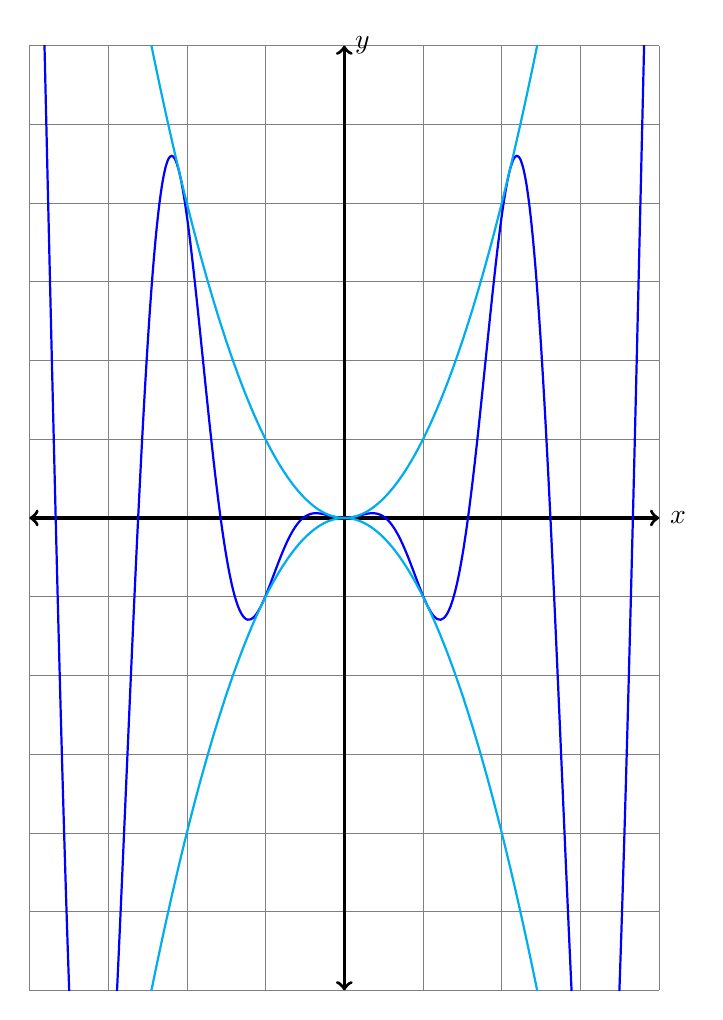
\begin{tikzpicture}
			\draw[very thin, gray] (-4, -6) grid (4, 6);
			\draw[very thick, <->] (-4, 0) -- (4, 0) node[right]{$x$};
			\draw[very thick, <->] (0, -6) -- (0, 6) node[right]{$y$};

			\clip (-4, -6) rectangle (4, 6);
			\draw[thick, blue, variable=\x, smooth, samples=200, domain=-4:4]
			plot ({\x}, {\x * \x * cos(3 * \x r)});

			\draw [thick, cyan, variable=\x, smooth, samples=200, domain=-4:4]
			plot({\x}, {\x * \x});
			\draw [thick, cyan, variable=\x, smooth, samples=200, domain=-4:4]
			plot({\x}, {-\x * \x});

		\end{tikzpicture}
	\end{center}

	برای قسمت موهومی:
	\begin{equation*}
		Im\{x(t)\} = j(t^2 \sin(3t))
	\end{equation*}

	و مشابه نمودار قبلی، نمودار آن همان نمودار
	$\sin(3t)$
	است که دامنه آن به صورت سهموی از دو طرف رشد می‌کند.

	\begin{center}
		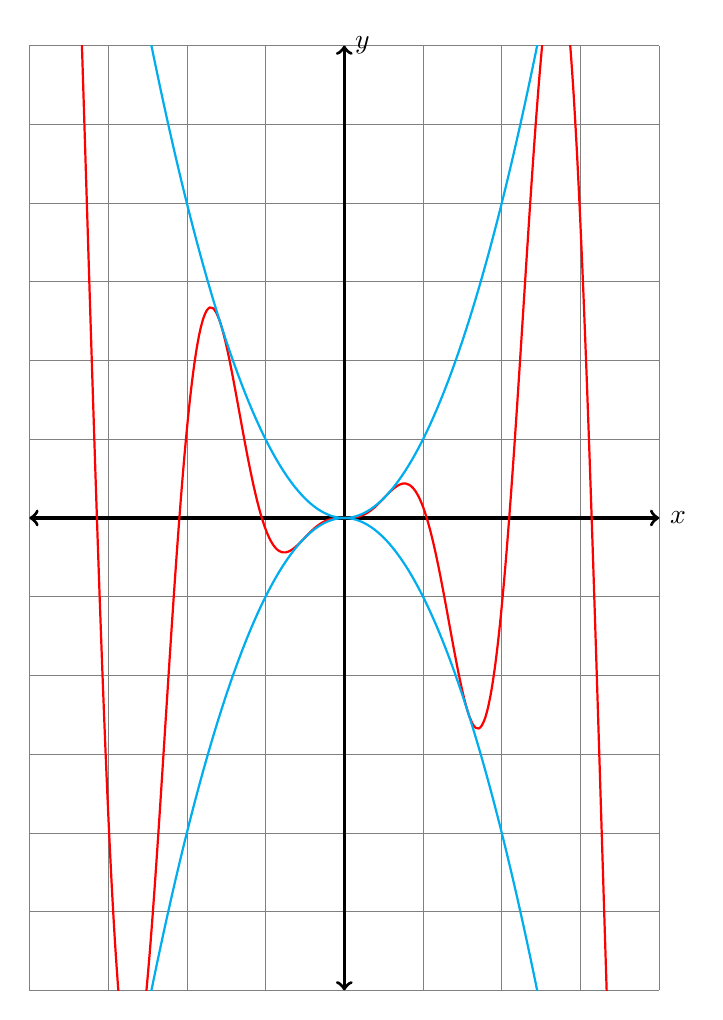
\begin{tikzpicture}
			\draw[very thin, gray] (-4, -6) grid (4, 6);
			\draw[very thick, <->] (-4, 0) -- (4, 0) node[right]{$x$};
			\draw[very thick, <->] (0, -6) -- (0, 6) node[right]{$y$};

			\clip (-4, -6) rectangle (4, 6);
			\draw[thick, red, variable=\x, smooth, samples=200, domain=-4:4]
			plot ({\x}, {\x * \x * sin(3 * \x r)});

			\draw [thick, cyan, variable=\x, smooth, samples=200, domain=-4:4]
			plot({\x}, {\x * \x});
			\draw [thick, cyan, variable=\x, smooth, samples=200, domain=-4:4]
			plot({\x}, {-\x * \x});

		\end{tikzpicture}
	\end{center}

	برای نمودار شکل مزدوج نیز کافیست نمودار قسمت موهومی را نسبت به محور
	$x$
	قرینه کنیم (نمودار قسمت حقیقی تفاوتی نخواهد کرد):

	\begin{center}
		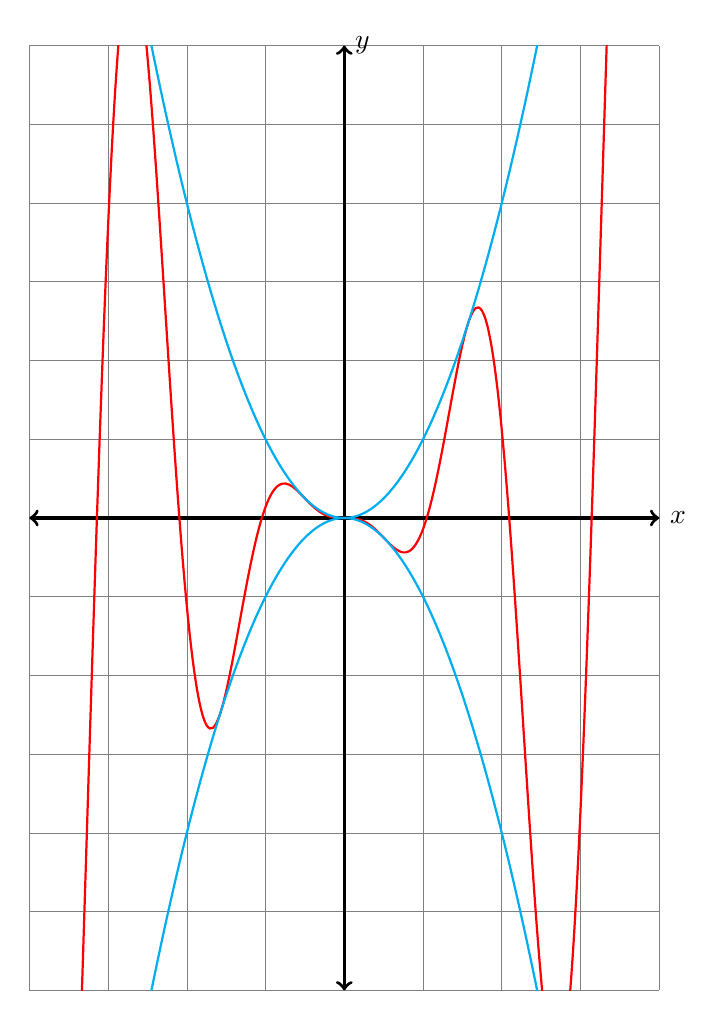
\begin{tikzpicture}
			\draw[very thin, gray] (-4, -6) grid (4, 6);
			\draw[very thick, <->] (-4, 0) -- (4, 0) node[right]{$x$};
			\draw[very thick, <->] (0, -6) -- (0, 6) node[right]{$y$};

			\clip (-4, -6) rectangle (4, 6);
			\draw[thick, red, variable=\x, smooth, samples=200, domain=-4:4]
			plot ({\x}, {- \x * \x * sin(3 * \x r)});

			\draw [thick, cyan, variable=\x, smooth, samples=200, domain=-4:4]
			plot({\x}, {\x * \x});
			\draw [thick, cyan, variable=\x, smooth, samples=200, domain=-4:4]
			plot({\x}, {-\x * \x});

		\end{tikzpicture}
	\end{center}

	\subsection*{ب)}
	\paragraph*{}
	برای قسمت حقیقی
	$y(t)$:

	\begin{equation*}
		Re\{y(t)\} = \Pi(\frac{t}{2}) =
		\begin{cases}
			\begin{matrix}
				1 & |t| < 1 \\
				0 & o.w.
			\end{matrix}
		\end{cases}
	\end{equation*}

	\begin{center}
		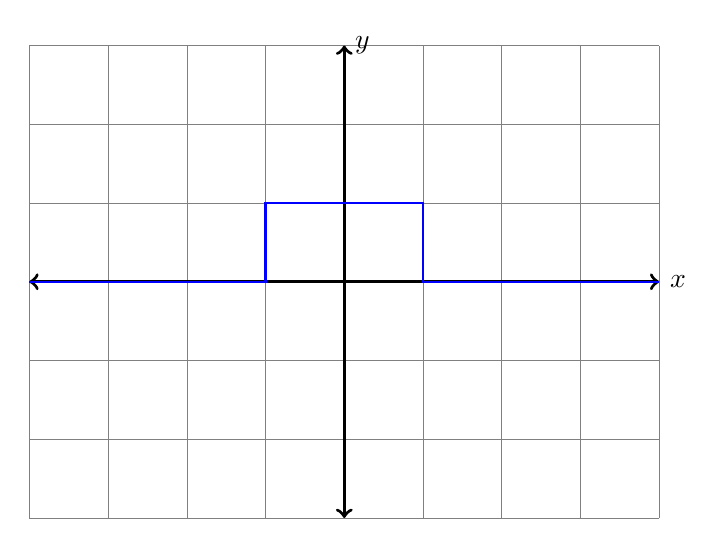
\begin{tikzpicture}
			\draw[very thin, gray] (-4, -3) grid (4, 3);
			\draw[very thick, <->] (-4, 0) -- (4, 0) node[right]{$x$};
			\draw[very thick, <->] (0, -3) -- (0, 3) node[right]{$y$};

			\draw[thick, blue] (-4, 0) -- (-1, 0) -- (-1, 1) -- (1, 1) -- (1, 0) -- (4, 0);
		\end{tikzpicture}
	\end{center}

	برای قسمت موهومی:
	\begin{equation*}
		Im\{y(t)\} = \Lambda (t) =
		\begin{cases}
			\begin{matrix}
				1 - |t| & |t| < 1 \\
				0 & o.w.
			\end{matrix}
		\end{cases}
	\end{equation*}

	\begin{center}
		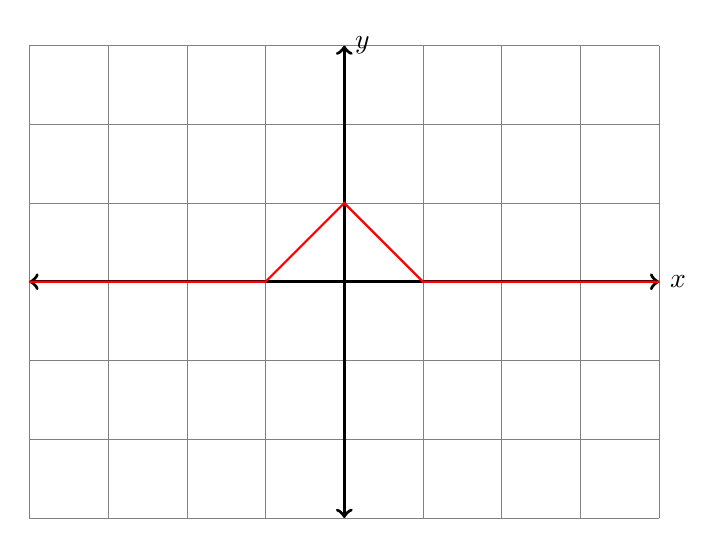
\begin{tikzpicture}
			\draw[very thin, gray] (-4, -3) grid (4, 3);
			\draw[very thick, <->] (-4, 0) -- (4, 0) node[right]{$x$};
			\draw[very thick, <->] (0, -3) -- (0, 3) node[right]{$y$};

			\draw[thick, red] (-4, 0) -- (-1, 0) -- (0, 1) -- (1, 0) -- (4, 0);
		\end{tikzpicture}
	\end{center}


	\subsection*{ج)}
	\paragraph*{}
	داریم:
	\begin{equation*}
		\Pi(t) =
		\begin{cases}
			\begin{matrix}
				1 & |t| < \frac{1}{2}\\
				0 & o.w.
			\end{matrix}
		\end{cases}
	\end{equation*}

	بنابراین برای رسم نمودار سیگنال
	$z(t) = \Pi(\frac{t}{2} - \frac{1}{2})$
	کافیست نمودار
	$\Pi(t)$
	را
	$\frac{1}{2}$
	واحد به راست جابه‌جا کرده:

	\begin{center}
		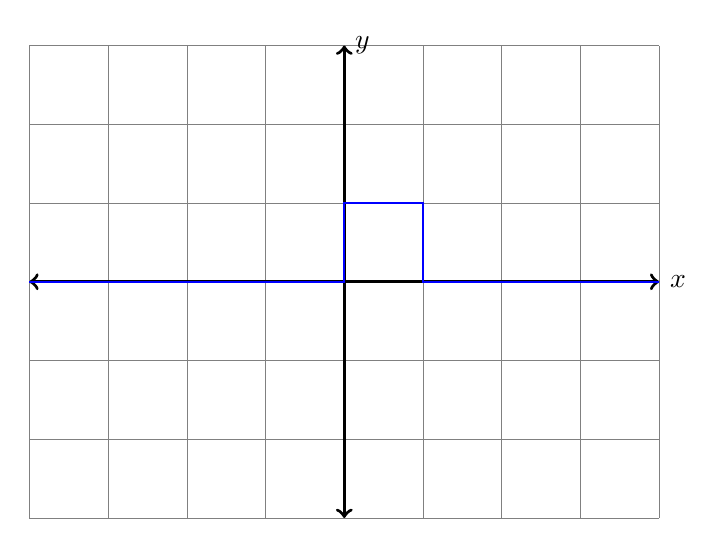
\begin{tikzpicture}
			\draw[very thin, gray] (-4, -3) grid (4, 3);
			\draw[very thick, <->] (-4, 0) -- (4, 0) node[right]{$x$};
			\draw[very thick, <->] (0, -3) -- (0, 3) node[right]{$y$};

			\draw[thick, blue] (-4, 0) -- (0, 0) -- (0, 1) -- (1, 1) -- (1, 0) -- (4, 0);
		\end{tikzpicture}
	\end{center}

	و x هر نقطه را دو برابر کنیم:

	\begin{center}
		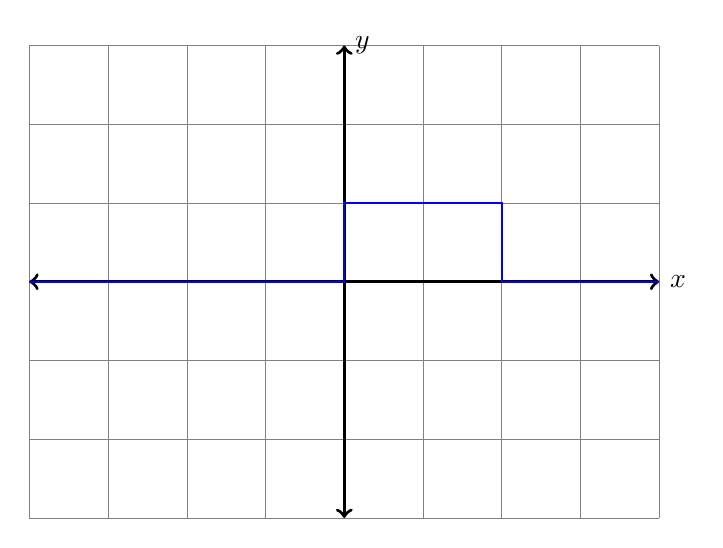
\begin{tikzpicture}
			\draw[very thin, gray] (-4, -3) grid (4, 3);
			\draw[very thick, <->] (-4, 0) -- (4, 0) node[right]{$x$};
			\draw[very thick, <->] (0, -3) -- (0, 3) node[right]{$y$};

			\draw[thick, blue] (-4, 0) -- (0, 0) -- (0, 1) -- (2, 1) -- (2, 0) -- (4, 0);
		\end{tikzpicture}
	\end{center}

	با توجه به این که سیگنال حقیقی‌مقدار است، قسمت موهومی سیگنال ثابت صفر است (یا به عبارتی
	$Im\{z(t)\} = 0$).
	بنابراین شکل قسمت موهومی سیگنال
	$z$
	و
	$z^*$
	یکسان خواهد بود.

\end{document}